% !TeX root = ../Book3.tex
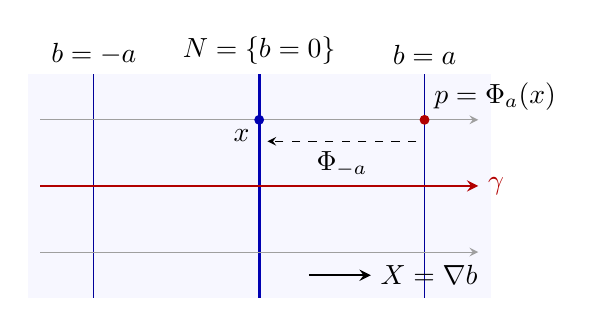
\begin{tikzpicture}[>=stealth,scale=1.05]
	\fill[blue!3] (-2.8,-1.35) rectangle (2.8,1.35);
	\draw[blue!60!black] (-2,-1.35)--(-2,1.35);
	\draw[very thick,blue!70!black] (0,-1.35)--(0,1.35);
	\draw[blue!60!black] (2,-1.35)--(2,1.35);
	\node[above] at (-2,1.35) {\(b=-a\)};
	\node[above] at (0,1.35) {\(N=\{b=0\}\)};
	\node[above] at (2,1.35) {\(b=a\)};
	\draw[->,gray!75] (-2.65,-.8)--(2.65,-.8);
	\draw[->,thick,red!70!black] (-2.65,0)--(2.65,0);
	\node[right,red!70!black] at (2.65,0) {\(\gamma\)};
	\draw[->,gray!75] (-2.65,.8)--(2.65,.8);
	\fill[blue!70!black] (0,.8) circle (1.7pt);
	\fill[red!70!black] (2,.8) circle (1.7pt);
	\node[below left] at (0,.8) {\(x\)};
	\node[above right] at (2,.8) {\(p=\Phi_a(x)\)};
	\draw[->,dashed] (1.9,.54)--(.1,.54);
	\node[below] at (1,.54) {\(\Phi_{-a}\)};
	\draw[->,thick] (.6,-1.08)--(1.35,-1.08);
	\node[right] at (1.35,-1.08) {\(X=\nabla b\)};
\end{tikzpicture}
